\documentclass[11pt,a4paper]{article}

% ---------------------------------------------------------------
%  ILAC-WAN Extension Study -- Version 2.0 (Consolidated Roadmap)
% ---------------------------------------------------------------
\usepackage[T1]{fontenc}
\usepackage[utf8]{inputenc}
\usepackage{mathptmx}
\usepackage{microtype}
\usepackage[a4paper,top=2.3cm,bottom=2.5cm,left=2.2cm,right=2.2cm]{geometry}
\usepackage{amsmath,amssymb,amsthm,bm}
\usepackage{graphicx}
\usepackage{xcolor}
\usepackage{booktabs}
\usepackage{array}
\usepackage{longtable}
\usepackage{multirow}
\usepackage{enumitem}
\usepackage{titlesec}
\usepackage{fancyhdr}
\usepackage{lastpage}
\usepackage{caption}
\usepackage{tikz}
\usetikzlibrary{arrows.meta,positioning,calc,shapes.misc,decorations.pathreplacing}
\usepackage[most]{tcolorbox}
\usepackage[hidelinks]{hyperref}
\hypersetup{colorlinks=true,linkcolor=accent,citecolor=okgreen,urlcolor=accent2}

% ----------------------------- colors ----------------------------
\definecolor{accent}{RGB}{13,59,102}    % deep petrol blue
\definecolor{accent2}{RGB}{14,116,144}  % teal
\definecolor{okgreen}{RGB}{21,107,64}
\definecolor{brick}{RGB}{154,32,32}
\definecolor{gold}{RGB}{176,124,11}
\definecolor{paleblue}{RGB}{242,247,251}
\definecolor{palegreen}{RGB}{242,250,245}
\definecolor{palered}{RGB}{252,244,244}
\definecolor{palegold}{RGB}{252,249,240}

% --------------------------- typography ---------------------------
\titleformat{\section}{\Large\bfseries\color{accent}}{\thesection}{0.7em}{}[{\vspace{-0.5ex}\color{accent}\rule{\textwidth}{0.9pt}}]
\titleformat{\subsection}{\large\bfseries\color{accent2}}{\thesubsection}{0.6em}{}
\titleformat{\subsubsection}{\normalsize\bfseries\color{accent}}{\thesubsubsection}{0.6em}{}
\titlespacing*{\section}{0pt}{1.4em}{0.9em}
\titlespacing*{\subsection}{0pt}{1.1em}{0.5em}

\pagestyle{fancy}
\fancyhf{}
\renewcommand{\headrulewidth}{0.6pt}
\renewcommand{\headrule}{\hbox to\headwidth{\color{accent}\leaders\hrule height \headrulewidth\hfill}}
\fancyhead[L]{\small\color{accent}\textbf{ILAC--WAN Extension Study --- v2.0}}
\fancyhead[R]{\small\color{accent}Critical Audit \& Research Roadmap}
\fancyfoot[C]{\small Page \thepage\ of \pageref{LastPage}}

% ----------------------------- boxes ------------------------------
\newtcolorbox{limitbox}[1]{enhanced,breakable,colback=palered,colframe=brick,
  fonttitle=\bfseries\small,title={#1},boxrule=0.8pt,arc=1.5pt,
  left=7pt,right=7pt,top=5pt,bottom=5pt}
\newtcolorbox{ideabox}[1]{enhanced,breakable,colback=palegreen,colframe=okgreen,
  fonttitle=\bfseries\small,title={#1},boxrule=0.8pt,arc=1.5pt,
  left=7pt,right=7pt,top=5pt,bottom=5pt}
\newtcolorbox{infobox}[1]{enhanced,breakable,colback=paleblue,colframe=accent,
  fonttitle=\bfseries\small,title={#1},boxrule=0.8pt,arc=1.5pt,
  left=7pt,right=7pt,top=5pt,bottom=5pt}
\newtcolorbox{goldbox}[1]{enhanced,breakable,colback=palegold,colframe=gold,
  fonttitle=\bfseries\small,title={#1},boxrule=0.8pt,arc=1.5pt,
  left=7pt,right=7pt,top=5pt,bottom=5pt}

\newtheorem{proposition}{Proposition}
\newtheorem{remark}{Remark}

\newcommand{\Ltag}[1]{\textcolor{brick}{\textbf{#1}}}
\newcommand{\Dir}[1]{\textcolor{accent}{\textbf{Direction~#1}}}
\setlist{itemsep=2pt,topsep=3pt,parsep=0pt}
\setlength{\parskip}{2pt}

\begin{document}

% ============================ TITLE PAGE ============================
\begin{titlepage}
\thispagestyle{empty}
\begin{center}
{\color{accent}\rule{\textwidth}{2.2pt}}\\[0.35em]
{\color{accent2}\rule{\textwidth}{0.7pt}}

\vspace{1.6cm}
{\small\scshape B.\,Tech.\ Project --- Consolidated Technical Proposal, Critical Audit \& Execution Roadmap}\\[0.25em]
{\small\color{gold}\bfseries Version 2.0 \,---\, supersedes and extends the v1 proposal of 6 June 2026}

\vspace{1.1cm}
{\Huge\bfseries\color{accent} Fidelity-Aware, Learning-Augmented,\\[0.25em] and Trust-Resilient Wireless\\[0.25em] Agent Networks}\\[0.8em]
{\Large\color{black} A Twenty-Three-Point Limitation Audit and Five Ranked,\\ Falsifiable Research Directions for the Progressive Knowledge\\ Aggregation Framework under ILAC}

\vspace{1.2cm}
\begin{tcolorbox}[colback=paleblue,colframe=accent,boxrule=0.8pt,arc=2pt,width=0.92\textwidth]
\small\textbf{Reference paper under study:}\\[2pt]
Z.~Zhao, J.~Wang, Z.~Yang, K.~Yang, Z.~Zhang, M.~Chen, and K.~Huang, ``Agentic AI--Empowered Wireless Agent Networks With Semantic-Aware Collaboration via ILAC,'' \emph{arXiv:2604.02381}, 2026.
\end{tcolorbox}

\vspace{1.0cm}
\renewcommand{\arraystretch}{1.35}
\begin{tabular}{r p{8.6cm}}
\textbf{Submitted by:} & [Student Name] \quad\textbar\quad [Enrolment Number] \\
\textbf{Programme:} & B.\,Tech., Information Technology \\
\textbf{Institute:} & Atal Bihari Vajpayee Indian Institute of Information Technology and Management (ABV--IIITM), Gwalior \\
\textbf{Supervisor:} & [Professor Name] \\
\textbf{Date:} & June 2026 \qquad \textbf{Duration:} two months (eight weeks) \\
\end{tabular}

\vfill
\begin{tcolorbox}[colback=palegold,colframe=gold,boxrule=0.8pt,arc=2pt,width=0.92\textwidth]
\footnotesize\textbf{What is new in v2.0.}\; (i) The limitation audit grows from eleven to \textbf{twenty-three} equation-anchored items, now including \textbf{five internal inconsistencies} (v1 had three); the two strongest --- a violation of Wyner--Ziv side-information coding at the link level (L18) and a lookahead that never shapes the continuous decisions (L19) --- were found in this revision. (ii) The five directions are \textbf{re-ranked and re-verified} against the 2025--2026 literature; a new trust-resilient direction enters at rank~3. (iii) Directions~1 and~2 are upgraded into detailed, week-mapped blueprints integrating \textbf{Wyner--Ziv conditional coding, conformal risk control, decision-focused learning through the exact matcher, a Lyapunov control baseline,} and a \textbf{provably dominant flexible scheduling action space}. Every headline claim carries a falsifiable success target measured against the paper's own baselines.
\end{tcolorbox}

\vspace{0.5cm}
{\color{accent2}\rule{\textwidth}{0.7pt}}\\[0.3em]
{\color{accent}\rule{\textwidth}{2.2pt}}
\end{center}
\end{titlepage}

% ========================= EXECUTIVE SUMMARY ========================
\section*{Executive Summary}
\addcontentsline{toc}{section}{Executive Summary}

The reference paper proposes a \emph{wireless agent network} (WAN) in which mobile, embodied-large-model (ELM) agents perform \emph{progressive knowledge aggregation}: distributed sensory data is pairwise fused, de-duplicated, and semantically compressed as it climbs a dynamically formed topology toward a single root, minimising total mobility, computation, and communication energy. The framework is solved by the two-level \mbox{H--MAP} algorithm: a convex inner level (BCD over a resource block and an SCA-convexified motion block) and a potential-field-guided minimum-weight perfect matching (Edmonds' Blossom) at the outer level.

This document is the consolidated v2.0 of the project proposal. It contains: \textbf{(a)} a complete restatement of the framework; \textbf{(b)} a three-tier, twenty-three-point limitation audit in which every item is anchored to a specific equation, constraint, or algorithm line --- Tier~I reproduces the v1 audit (L1--L11), Tier~II adds six structural gaps uncovered by a literature-grounded re-examination (L12--L17), and Tier~III adds six findings from a second close read of the mathematics (L18--L23), including two new internal inconsistencies; \textbf{(c)} five ranked research directions, each with methodology, mathematics, tools, evaluation plan, and an explicit falsifiable success target; \textbf{(d)} fully detailed blueprints for the recommended pair, \Dir{1} (fidelity-aware aggregation grounded in CEO/Wyner--Ziv theory with conformal certification) and \Dir{2} (a learned, decision-focused predictive topology over a provably enlarged action space); and \textbf{(e)} an eight-week execution plan, a risk register with guaranteed floors, and a publication outlook.

\begin{infobox}{The two sentences that define this project}
\emph{First}, the reference framework treats lossy semantic compression as free and the radio link as ignorant of the receiver's knowledge; restoring fidelity (rate--distortion/CEO) and side information (Wyner--Ziv) overturns its published trivial optimum $\eta^{\star}=\eta^{\mathrm{req}}$ and yields a certified energy--fidelity frontier. \emph{Second}, its ``predictive'' topology rests on a hand-tuned, internally inconsistent one-step heuristic; replacing it with a learned, decision-focused cost-to-go over a strictly larger scheduling action space dominates the published algorithm by construction and scales to network sizes the paper never reaches.
\end{infobox}

\clearpage
\tableofcontents
\clearpage

% =========================== 1. INTRODUCTION ========================
\section{Introduction and Motivation}

Sixth-generation (6G) research is shifting from connecting devices to connecting \emph{autonomous intelligences}. Foundation-model-equipped agents that sense, reason, and act --- \emph{agentic AI} --- motivate the Internet of Agents, in which the network's purpose becomes high-level knowledge sharing rather than raw bit transport. The reference paper situates itself in this trend under \emph{integrated learning and communication} (ILAC) and contributes a genuinely valuable artefact: a single mathematical model in which agent mobility, ELM-based semantic processing, and wireless transmission are jointly optimised for a surveillance-style aggregation mission, solved by a clean hierarchical algorithm with an $\mathcal{O}(N^{3})$ complexity claim and a reported $\sim$19\% energy gain over a distance-based topology at $N{=}10$.

Precisely because the model is clean, its assumptions are cleanly attackable. The purpose of this project is to convert that attack surface into a defensible B.\,Tech.\ project and, realistically, one to two publishable manuscripts. The governing philosophy of this proposal is \textbf{falsifiability}: every proposed contribution is stated together with the concrete experiment, baseline, and number that would confirm or refute it, and every extension deliberately reuses the paper's own benchmark suite so that all comparisons are like-for-like.

Relative to the v1 proposal, this revision is the product of two additional passes: a literature-grounded re-examination against the 2025--2026 state of the art (token/KV-cache agent communication, Byzantine-robust multi-agent LLM systems, conformal reliability for wireless AI, decision-focused learning, over-the-air computation, and rate--distortion-optimised collaborative perception), and a second equation-by-equation read of the paper that surfaced previously uncaught internal inconsistencies. Both passes \emph{strengthened} rather than displaced the original top-ranked directions; the audit below explains why.

% ====================== 2. REFERENCE FRAMEWORK ======================
\section{Overview of the Reference Framework}
\label{sec:framework}

\subsection{System model}
A set $\mathcal{N}=\{1,\dots,N\}$ of mobile agents patrols circular regions; agent $i$'s position obeys the hard coverage constraint $\lVert \mathbf p_i-\mathbf c_i\rVert_2\le R_i$ (Eq.~(1)). Aggregation proceeds in synchronous rounds $k=1,\dots,K$ with $K=\lceil\log_2 N\rceil$. The \emph{information source state} $\Omega_i^{(k)}\subseteq\mathcal N$ records whose original data agent $i$ holds and evolves by set union; the payload evolves by the \emph{additive fusion rule}
\begin{equation}
L_j^{(k+1)}=\eta_j L_j^{(k)}+\eta_i L_i^{(k)},\qquad \eta_u=\frac{L_u^{(k+1)}}{L_u^{(k)}}\in(0,1],
\label{eq:fusion}
\end{equation}
where $\eta_u$ is the semantic compression ratio (paper Eqs.~(2),(7)). Semantic overlap is proxied \emph{geometrically} by the Jaccard similarity $\rho^{(k)}_{u,v}$ of accumulated patrol-area unions (Eq.~(5)), and it discounts only the \emph{compute} cost (in FLOPs)
\begin{equation}
W^{\mathrm{comp}}_u=L_u^{(k)}\Big[C_{\mathrm{base}}+C_{\mathrm{gen}}\gamma\big(1-\rho^{(k)}_{u,v}\big)\ln\tfrac{1}{\eta_u}\Big],
\qquad E_u^{\mathrm{comp}}=\tau f_u^2 W_u^{\mathrm{comp}},
\label{eq:comp}
\end{equation}
with $\rho$ measured against the agent's \emph{predecessor} from round $k{-}1$. Mobility follows a polynomial power model; the channel is pure large-scale path loss $h_{ij}=\beta_0\lVert\mathbf p_i-\mathbf p_j\rVert_2^{-\delta}$ with Shannon-rate transmission over \emph{orthogonal} channels; the transmitted payload is $D_i^{\mathrm{out}}=\eta_i L_i^{(k)}$ regardless of the receiver's knowledge.

\subsection{Problem formulation and the H--MAP algorithm}
The \textbf{inner level} (P1) minimises the pairwise interaction energy $E^{\mathrm{total}}_{(i,j)}=E^{\mathrm{mob}}_i+E^{\mathrm{mob}}_j+E^{\mathrm{comp}}_i+E^{\mathrm{comp}}_j+E^{\mathrm{comm}}_i$ over positions, velocities, transmit power, and compression ratios, subject to the coverage constraint, a per-round latency deadline $T_{\max}$, and box constraints; it is solved by BCD (a provably convex resource block solved by 1-D bisection, and an SCA/SOCP motion block). The published inner-level conclusion is that the receiver's optimum sits on its bound, $\eta_j^{\star}=\eta_j^{\mathrm{req}}$. The \textbf{outer level} (P2) selects binary pairings $\alpha^{(k)}_{i,j}$ to minimise cumulative energy under the constraints that each active agent appears in at most one link per round (Eq.~(16a)) and that \emph{exactly} $M^{(k)}=\lfloor N^{(k)}/2\rfloor$ pairs form per round (Eq.~(16b), ``maximum parallelism''). H--MAP solves each round as a minimum-weight perfect matching on an augmented graph (a virtual node absorbs an odd agent) with edge weights
\begin{equation}
w^{(k)}_{i,j}=W^{(k)}_{i,j}+\Phi^{(k)}_j,\qquad
\Phi^{(k)}_j=\zeta\,\big\lVert \mathbf p^{\mathrm{end}}_j-\bar{\mathbf P}^{(k)}_c\big\rVert_2^{\delta}\cdot L_j^{(k+1)},
\label{eq:potential}
\end{equation}
where $\bar{\mathbf P}^{(k)}_c$ is the active-set centroid and $\zeta$ a hand-tuned weight; directed weights are symmetrised as $\tilde w_{ij}=\min(w_{ij},w_{ji})$ before Blossom matching, and the direction is restored afterwards.

\begin{figure}[t]
\centering
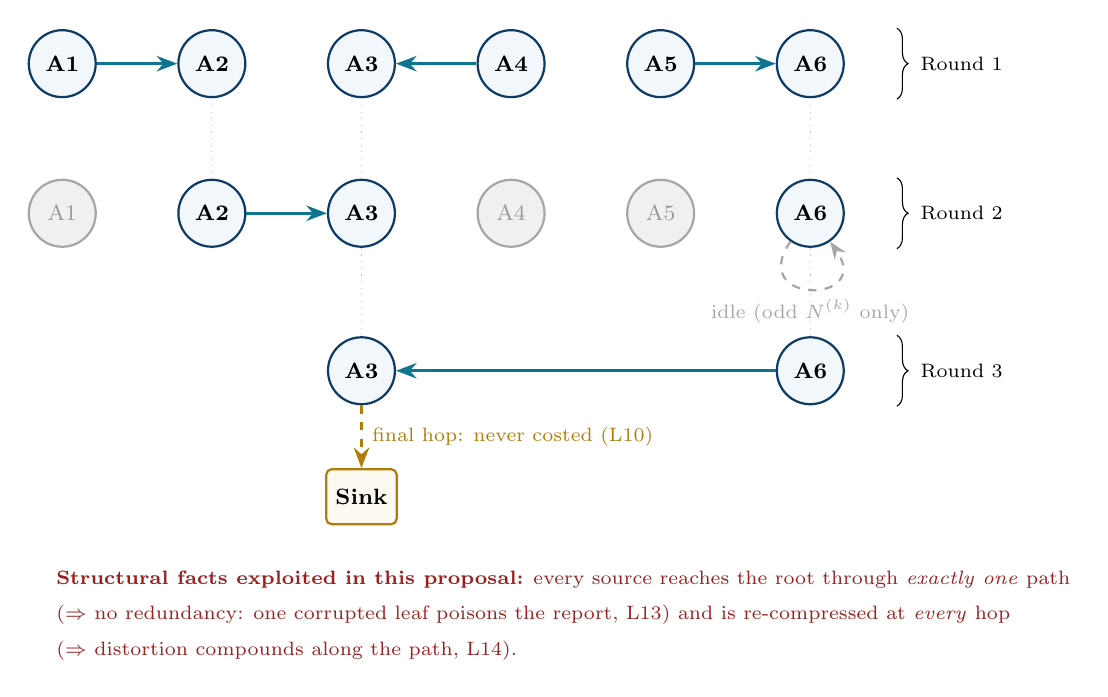
\begin{tikzpicture}[
  agent/.style={circle,draw=accent,fill=paleblue,thick,minimum size=8.5mm,font=\footnotesize\bfseries},
  retired/.style={circle,draw=gray!70,fill=gray!12,thick,minimum size=8.5mm,font=\footnotesize,text=gray!80},
  lnk/.style={-{Stealth[length=2.6mm]},very thick,accent2},
  idle/.style={-{Stealth[length=2.2mm]},thick,gray!70,dashed},
  note/.style={font=\scriptsize,align=left}]
% round 1
\node[agent] (a1) at (0,0) {A1};
\node[agent] (a2) at (1.9,0) {A2};
\node[agent] (a3) at (3.8,0) {A3};
\node[agent] (a4) at (5.7,0) {A4};
\node[agent] (a5) at (7.6,0) {A5};
\node[agent] (a6) at (9.5,0) {A6};
\draw[lnk] (a1) -- (a2);
\draw[lnk] (a4) -- (a3);
\draw[lnk] (a5) -- (a6);
% round 2
\node[retired] (b1) at (0,-1.9) {A1};
\node[agent]   (b2) at (1.9,-1.9) {A2};
\node[agent]   (b3) at (3.8,-1.9) {A3};
\node[retired] (b4) at (5.7,-1.9) {A4};
\node[retired] (b5) at (7.6,-1.9) {A5};
\node[agent]   (b6) at (9.5,-1.9) {A6};
\draw[lnk] (b2) -- (b3);
\draw[idle] (b6) to[out=235,in=305,looseness=5] node[below,note]{idle (odd $N^{(k)}$ only)} (b6);
% round 3
\node[agent] (c3) at (3.8,-3.9) {A3};
\node[agent] (c6) at (9.5,-3.9) {A6};
\draw[lnk] (c6) -- (c3);
% root to sink
\node[draw=gold,fill=palegold,thick,rounded corners=2pt,minimum size=7mm,font=\footnotesize\bfseries] (sink) at (3.8,-5.5) {Sink};
\draw[-{Stealth[length=2.6mm]},very thick,gold,dashed] (c3) -- node[right,note,text=gold]{final hop: never costed (L10)} (sink);
% vertical guides
\draw[gray!50,dotted] (a2) -- (b2); \draw[gray!50,dotted] (a3) -- (b3); \draw[gray!50,dotted] (a6) -- (b6);
\draw[gray!50,dotted] (b3) -- (c3); \draw[gray!50,dotted] (b6) -- (c6);
% round braces
\draw[decorate,decoration={brace,amplitude=4pt}] (10.6,0.45) -- (10.6,-0.45) node[midway,right=5pt,note]{Round 1};
\draw[decorate,decoration={brace,amplitude=4pt}] (10.6,-1.45) -- (10.6,-2.35) node[midway,right=5pt,note]{Round 2};
\draw[decorate,decoration={brace,amplitude=4pt}] (10.6,-3.45) -- (10.6,-4.35) node[midway,right=5pt,note]{Round 3};
% annotation
\node[note,text=brick,anchor=west] at (-0.2,-6.55) {\textbf{Structural facts exploited in this proposal:} every source reaches the root through \emph{exactly one} path};
\node[note,text=brick,anchor=west] at (-0.2,-7.0) {($\Rightarrow$ no redundancy: one corrupted leaf poisons the report, L13) and is re-compressed at \emph{every} hop};
\node[note,text=brick,anchor=west] at (-0.2,-7.45) {($\Rightarrow$ distortion compounds along the path, L14).};
\end{tikzpicture}
\caption{Progressive knowledge aggregation as a converging forest ($N{=}6$). Greyed agents have ``retired'' after transmitting; the active set roughly halves each round until a single root remains.}
\label{fig:tree}
\end{figure}

% ===================== 3. LIMITATION AUDIT ==========================
\section{The Twenty-Three-Point Limitation Audit}
\label{sec:audit}

The audit is organised in three tiers reflecting how each finding was obtained. \textbf{Tier~I} (L1--L11) is the v1 audit, retained verbatim in condensed form. \textbf{Tier~II} (L12--L17) emerged from re-examining the framework against the 2025--2026 literature. \textbf{Tier~III} (L18--L23) emerged from a second, finer equation-by-equation read and contains the two strongest findings of this revision. Items are tagged by type: a \emph{gap} (something real is missing), an \emph{inconsistency} (the model contradicts its own premises), an \emph{artefact} (a degenerate consequence of a modelling choice), or a \emph{validation} issue. Five items are internal inconsistencies: \Ltag{L2}, \Ltag{L3}, \Ltag{L10}, \Ltag{L19}, \Ltag{L21}.

\subsection{Tier I --- the v1 audit in brief (L1--L11)}
\begin{table}[h]
\centering\footnotesize
\renewcommand{\arraystretch}{1.25}
\begin{tabular}{@{}c l p{8.6cm} l@{}}
\toprule
\textbf{ID} & \textbf{Anchor} & \textbf{Limitation (summary)} & \textbf{Targeted by} \\
\midrule
L1 & Eq.~(1) & No sensing-quality model; mobility serves only the radio channel. & \Dir{4} \\
L2 & Eq.~(12) & \emph{Inconsistency:} retired senders abandon their zones despite the ``continuous coverage'' mission. & \Dir{4} \\
L3 & Eq.~(2) & \emph{Inconsistency:} additive fusion ignores cross-redundancy; $\rho$ never shrinks the fused size. & \Dir{1} \\
L4 & Eq.~(5) & Semantic similarity is a purely geometric (Jaccard-of-areas) proxy. & \Dir{1} \\
L5 & Eq.~(6) & FLOPs/frequency ELM energy model; real LLM inference is memory-bound. & Cross-cutting \\
L6 & Eqs.~(8),(9) & Deterministic path-loss channel; no fading, shadowing, or outage. & \Dir{5} \\
L7 & Sec.~II-E & Unlimited orthogonal spectrum; interference assumed away. & Wildcard \\
L8 & Eq.~(14) & Energy-only objective; no fidelity, freshness, or value of information. & \Dir{1}, \Dir{3} \\
L9 & Eq.~(35), Fig.~7 & Hand-tuned, myopic potential field; energy rebounds when $\zeta$ is mis-set. & \Dir{2} \\
L10 & Alg.~2 & \emph{Inconsistency:} central hub uncosted; final root-to-sink hop never modelled. & \Dir{3}, Wildcard \\
L11 & Sec.~V & Validation at $N\le 10$, fully synthetic, no real ELM/RAG pipeline, no runtime. & All \\
\bottomrule
\end{tabular}
\caption{Tier I: the original eleven limitations (full derivations in the v1 proposal).}
\label{tab:tier1}
\end{table}

\subsection{Tier II --- structural and modelling gaps (L12--L17)}

\textbf{\Ltag{L12} Forced maximum parallelism / fixed depth (anchor: Eqs.~(16b), (37); type: gap).} Constraint (16b) mandates \emph{exactly} $\lfloor N^{(k)}/2\rfloor$ pairs per round, and the virtual idle node exists only when $N^{(k)}$ is odd. With an even active set, no agent may ever sit out a round, and Eq.~(16a) forbids relaying within a round. The minimum-depth schedule $K=\lceil\log_2 N\rceil$ is therefore an \emph{assumption presented as a formulation}: when $T_{\max}$ is loose, idling a badly placed pair for one round (or permitting a short chain) can strictly reduce total energy. The paper's feasible set is unnecessarily small --- a fact \Dir{2} converts into a dominance guarantee (Proposition~\ref{prop:dominance}).

\textbf{\Ltag{L13} No trust or integrity model (anchor: Sec.~II-B, Fig.~\ref{fig:tree}; type: gap).} The state $\Omega$ records \emph{who} contributed but never \emph{whether the content is reliable}. Because the topology is a converging tree in which each source traverses exactly one path and senders retire after transmitting, a single hallucinated or poisoned payload at any leaf deterministically contaminates the global report --- there is zero redundancy. The 2025--2026 security literature identifies exactly this pattern --- propagation and amplification of semantic corruption through networked aggregation, and Byzantine behaviour in LLM multi-agent systems --- as a distinct, underexplored attack surface \cite{securesemcom,sacbyz,decentllm}. Targeted by \Dir{3}.

\textbf{\Ltag{L14} Compounding re-compression along the tree (anchor: Eq.~(2); type: gap).} A leaf's data is re-encoded once per round it is carried, so the effective end-to-end compression applied to source $s$'s information is the \emph{product} $\tilde\eta_s=\prod_{(u\to v)\in\mathcal P_s}\eta_u$ along its path $\mathcal P_s$ --- up to $K=\lceil\log_2 N\rceil$ successive lossy operations --- yet no model quantity tracks the cascade (a ``semantic telephone game''). This sharpens \Dir{1}: the distortion state must be path-multiplicative, which makes the interior-optimum result strictly stronger.

\textbf{\Ltag{L15} Bit-level payload abstraction is already dated for LLM agents (anchor: Eqs.~(2),(7),(10); type: gap).} The inter-agent payload is a scalar bit count scaled by $\eta$, while the 2025--2026 frontier of agent-to-agent communication is token-, latent-, and KV-cache-level exchange: tokens as the units of generative semantic communication \cite{tokcom}, learned machine-language token vocabularies for task-oriented agent links \cite{mltok}, and direct hidden-state/KV-cache transfer between models \cite{c2c,latentsurvey}. Re-expressing payloads in tokens (and energy in mJ/token, cf.\ L5) is a cheap modernisation adopted as a cross-cutting enhancement.

\textbf{\Ltag{L16} Sum-energy objective; batteries and reception ignored (anchor: Eqs.~(11),(14); type: gap).} Only the sender's transmit energy is counted (reception and decoding are free), and minimising the \emph{sum} can drain a single bottleneck agent --- typically a late-round receiver that fuses everything. No per-agent budget, no min--max/lifetime objective. Adopted as a one-paragraph objective variant in the evaluation plan.

\textbf{\Ltag{L17} One-shot episode versus continuous surveillance (anchor: Sec.~II-A; type: gap).} The formulation runs a single aggregation episode, whereas surveillance is a recurring process with data arrivals --- which is what makes Age-of-Information the natural complementary metric \cite{aoi}. Folded into \Dir{3}'s value-aware weighting and the future-work statement.

\subsection{Tier III --- second-pass findings (L18--L23)}

\begin{limitbox}{L18 --- Receiver side information never reduces the over-the-air payload (anchor: Eqs.~(5),(6),(10); type: gap; the sharpest finding of this revision)}
The correlation $\rho$ is defined only between an agent and its \emph{predecessor} from round $k{-}1$ and discounts only the \emph{compute} cost in Eq.~\eqref{eq:comp}. The transmitted payload in Eq.~(10) is $\eta_i L_i^{(k)}$ \emph{regardless of what the receiver $j$ already knows} --- even when $\Omega_j$ overlaps heavily with $\Omega_i$. This contradicts five decades of source-coding theory: with correlated side information $Z$ at the decoder, the Wyner--Ziv rate
\begin{equation}
R_{X|Z}(D)=\min_{T:\,T\!-\!X\!-\!Z}\; I(X;T\,|\,Z)
\label{eq:wz}
\end{equation}
is achievable and strictly smaller than the unconditional rate \cite{wynerziv}. Semantic communication is actively absorbing this principle right now --- learned side information at the receiver \cite{semantic_ic}, NN-based Wyner--Ziv encoders against shared codebooks \cite{wzcodebook}, and rate--distortion--perception treatments with explicit encoder/decoder side information \cite{rdpsem}. Bonus structure: $H(X_i|X_j)\ne H(X_j|X_i)$, so link costs are \emph{inherently asymmetric} --- finally a principled reason to retain the directed weights that the paper destroys via $\tilde w_{ij}=\min(w_{ij},w_{ji})$.
\end{limitbox}

\begin{limitbox}{L19 --- The lookahead never shapes the continuous decisions (anchor: Alg.~1 vs.\ Eq.~(36); type: \emph{internal inconsistency})}
Algorithm~1 minimises only the current-round energy of problem (P1); the potential field $\Phi$ in Eq.~\eqref{eq:potential} is then evaluated \emph{post hoc} at positions $\mathbf p^{\mathrm{end}\star}$ that were optimised \emph{without} $\Phi$. The framework's headline ``predictive'' mechanism thus influences only \emph{which pairs are selected}, never \emph{where agents actually move}: if converging toward the centroid genuinely lowers future cost, the motion planner is never incentivised to do it. The inner and outer levels optimise two mutually inconsistent objectives. \Dir{2} converts this into a free algorithm: moving $\Phi$ \emph{inside} (P1) --- which is convexity-preserving, see Remark~\ref{rem:phiconvex} --- yields a ``$\Phi$-in-the-loop'' H--MAP that should outperform the published method before any learning is introduced.
\end{limitbox}

\textbf{\Ltag{L20} Round-1 semantic encoding is free (anchor: $\rho^{(1)}_i{=}1$ with Eq.~(6); type: artefact).} Setting $\rho^{(1)}=1$ collapses Eq.~\eqref{eq:comp} to $W=L\,C_{\mathrm{base}}$, \emph{independent of $\eta$}: compressing raw sensory data into semantics --- in reality the single most expensive ELM operation (the VLM encoder pass) --- costs nothing extra at any depth, so round-1 agents should always compress maximally for free. This compounds the trivial-optimum problem attacked by \Dir{1} and further motivates the per-token energy repair of L5/L15.

\textbf{\Ltag{L21} Stale centroid (anchor: Eq.~(34); type: minor inconsistency).} $\bar{\mathbf P}_c^{(k)}$ averages over the \emph{current} active set --- including the senders who retire this very round --- so the ``future'' anchor is computed from a population half of which will not exist next round. The survivor centroid is the coherent target; even as a one-step predictor the heuristic is not internally consistent.

\textbf{\Ltag{L22} Synchronous lockstep rounds (anchor: Eq.~(15b); type: gap).} Every round is budgeted at $T_{\max}$, so mission latency is frozen at $K\,T_{\max}$, fast pairs idle-wait for slow ones, and no asynchronous or event-triggered operation is possible. Extends L12 and motivates the flexible action space of \Dir{2}.

\textbf{\Ltag{L23} $\eta^{\mathrm{req}}$ is exogenous (anchor: Eq.~(15f); type: gap).} The ``global directive to prevent payload explosion'' is handed to the optimiser from outside. Under \Dir{1}'s fidelity constraint it becomes \emph{derivable} from $(D_{\max},K)$ --- converting an arbitrary knob into a lemma.

\medskip
\noindent\textbf{Two rigor notes} (worth one line each in the final report): problem (P2) is written as if all future weights $W^{(k)}$ were known in advance, although they depend on realised states --- it is an MDP treated as a static program, which formally justifies \Dir{2}'s framing; and Theorem~1 claims \emph{strict} convexity while the proof establishes convexity only.

\subsection{Master mapping}
\begin{center}\footnotesize
\renewcommand{\arraystretch}{1.18}
\begin{longtable}{@{}c l p{6.9cm} l l@{}}
\toprule
\textbf{ID} & \textbf{Anchor} & \textbf{Summary} & \textbf{Type} & \textbf{Direction} \\
\midrule
\endhead
L1 & Eq.~(1) & No sensing-quality model & Gap & D4 \\
L2 & Eq.~(12) & Coverage hole on retirement & Inconsistency & D4 \\
L3 & Eq.~(2) & Additive fusion ignores redundancy & Inconsistency & D1 \\
L4 & Eq.~(5) & Geometric semantic proxy & Gap & D1 \\
L5 & Eq.~(6) & FLOPs-based ELM energy & Gap & Cross-cutting \\
L6 & Eqs.~(8),(9) & Deterministic channel, no outage & Gap & D5 \\
L7 & Sec.~II-E & Unlimited orthogonal spectrum & Gap & Wildcard \\
L8 & Eq.~(14) & Energy-only objective & Gap & D1, D3 \\
L9 & Eq.~(35) & Hand-tuned myopic potential field & Gap & D2 \\
L10 & Alg.~2 & Centralisation; final hop uncosted & Inconsistency & D3, Wildcard \\
L11 & Sec.~V & Small-scale synthetic validation & Validation & All \\
L12 & Eq.~(16b) & Forced max parallelism, fixed depth & Gap & D2 \\
L13 & Sec.~II-B & No trust/integrity; single-path tree & Gap & D3 \\
L14 & Eq.~(2) & Path-multiplicative re-compression untracked & Gap & D1 \\
L15 & Eqs.~(2),(10) & Bit-level abstraction vs.\ token/KV-cache reality & Gap & Cross-cutting \\
L16 & Eq.~(14) & Sum energy; batteries, reception ignored & Gap & Cross-cutting \\
L17 & Sec.~II-A & One-shot episode vs.\ continuous mission & Gap & D3 \\
L18 & Eq.~(10) & Wyner--Ziv side information violated at the link & Gap & D1 ($\to$D2) \\
L19 & Alg.~1/Eq.~(36) & Lookahead never shapes continuous decisions & Inconsistency & D2 \\
L20 & Eq.~(6) & Round-1 encoding free of $\eta$ & Artefact & D1, Cross-cutting \\
L21 & Eq.~(34) & Stale (pre-retirement) centroid & Inconsistency & D2 \\
L22 & Eq.~(15b) & Synchronous lockstep rounds & Gap & D2 \\
L23 & Eq.~(15f) & $\eta^{\mathrm{req}}$ exogenous, never derived & Gap & D1 \\
\bottomrule
\caption{All twenty-three audited limitations and the directions that target them.}
\label{tab:master}
\end{longtable}
\end{center}

% ===================== 4. RESEARCH DIRECTIONS =======================
\section{The Five Ranked Research Directions}
\label{sec:directions}

Each direction is self-contained, reuses the paper's own baselines so every claim is like-for-like comparable, and carries a falsifiable success target (consolidated in Section~\ref{sec:deliver}). Ranking criteria: guaranteed result floor, novelty, eight-week feasibility, machine-learning depth, and evaluation clarity. The ranking was \emph{re-verified twice}: every new Tier~II/III finding landed \emph{inside} Directions 1 and 2 and strengthened them, rather than pointing elsewhere.

% ----------------------------- D1 ---------------------------------
\subsection{Direction 1 (Rank 1) --- Fidelity-Aware Aggregation: CEO/Wyner--Ziv Theory with Conformal Certification}
\label{sec:d1}

\begin{limitbox}{Targets: L3, L4, L8, L14, L18, L20, L23}
Nothing in objective (14) penalises distortion, so the published inner-level optimum collapses to the trivial bound $\eta_j^{\star}=\eta_j^{\mathrm{req}}$: an agent may compress arbitrarily hard with no consequence for the global report. The fusion rule \eqref{eq:fusion} double-counts shared content (L3); the correlation proxy is purely geometric (L4); distortion compounds untracked along each source's path (L14); and the link rate ignores the receiver's side information in violation of Wyner--Ziv theory (L18).
\end{limitbox}

\begin{ideabox}{Key idea}
Re-cast WAN aggregation as a \emph{hierarchical CEO problem under logarithmic loss} \cite{ceo,courtade}: distributed encoders observe correlated noisy views of one true state $X$ and report over rate-limited links to a fusion centre under a distortion constraint. Introduce a path-multiplicative distortion state, a sub-additive fusion rule, and a side-information-aware payload; optimise energy \emph{subject to a fidelity floor}; certify the floor distribution-free with conformal risk control; and ground every modelling object ($\hat\rho$, $\Theta$) in measurements on a real collaborative-perception dataset.
\end{ideabox}

\subsubsection{Mathematical reformulation}
\textbf{(i) Distortion state.} Attach to each agent a distortion $D_i^{(k)}$, initialised losslessly ($D_i^{(1)}{=}0$) and updated on every fusion by a monotone, convex map in which harder compression never reduces distortion:
\begin{equation}
D_j^{(k+1)}=\Theta\big(D_j^{(k)},D_i^{(k)},\eta_i,\eta_j\big),\qquad \frac{\partial \Theta}{\partial \eta_u}\le 0 .
\label{eq:theta}
\end{equation}
Because of L14, $\Theta$ must respect path compounding: the information of source $s$ arrives at the root having experienced the product $\tilde\eta_s=\prod_{(u\to v)\in\mathcal P_s}\eta_u$, so root distortion is bounded through $\{\tilde\eta_s\}_{s\in\mathcal N}$, and under log-loss by the CEO conditional-entropy bound $D_{\mathrm{root}}\ge H(X\,|\,U_1,\dots,U_m,Q)$ \cite{courtade}.

\textbf{(ii) Sub-additive fusion (repairs L3).} Shared content is counted once:
\begin{equation}
L_j^{(k+1)}=\eta_j L_j^{(k)}+\eta_i L_i^{(k)}-\hat\rho_{ij}\,\min\big\{\eta_i L_i^{(k)},\,\eta_j L_j^{(k)}\big\}.
\label{eq:subadd}
\end{equation}

\textbf{(iii) Side-information-aware payload (repairs L18).} The over-the-air payload becomes conditional on the receiver's knowledge. Practical model and information-theoretic floor:
\begin{equation}
D_i^{\mathrm{out}}=\eta_i L_i^{(k)}\big(1-\omega\,\hat\rho_{ij}\big),
\qquad\text{floor: } R \;\ge\; R_{X_i|X_j}(D)=\!\!\min_{T:\,T-X_i-X_j}\! I(X_i;T\,|\,X_j),
\label{eq:condpayload}
\end{equation}
with $\omega\in[0,1]$ calibrated empirically (Sec.~\ref{sec:d1emp}). Since $H(X_i|X_j)\neq H(X_j|X_i)$, pairwise costs become \emph{asymmetric for a provable reason} --- consumed by \Dir{2}.

\textbf{(iv) Objective and endogenous $\eta^{\mathrm{req}}$ (repairs L8, L23).} Replace energy-only (14) by
\begin{equation}
\min_{\{\mathbf x\}} E^{\mathrm{total}}\;\;\text{s.t.}\;\;D_{\mathrm{root}}\le D_{\max}
\qquad\text{or}\qquad
\min_{\{\mathbf x\}} E^{\mathrm{total}}+\lambda\,D_{\mathrm{root}},
\label{eq:fidobj}
\end{equation}
and \emph{derive} the per-round compression bound as the largest compression compatible with the floor at depth $K$: $\eta^{\mathrm{req}}_j(k)=\sup\{\eta:\ \Theta\text{-forward bound at the root}\le D_{\max}\}$. Choosing $\Theta$ convex (e.g.\ log-loss-consistent) preserves the perspective-function convexity the paper exploits, so the BCD/SCA solver is \emph{extended, not discarded}. \textbf{Headline analytical result:} under \eqref{eq:fidobj} the optimum is \emph{interior}, $\eta^{\star}<\eta^{\mathrm{req}}$ in the binding regime --- overturning the published lemma-level conclusion.

\subsubsection{Certification layer: conformal risk control}
Rather than claiming $D_{\mathrm{root}}\le D_{\max}$ merely on average, the learned distortion map $\hat\Theta$ is calibrated on a held-out split so the guarantee holds \emph{distribution-free}: select the operating parameter (e.g.\ $\lambda$ or the compression schedule) by Learn-then-Test / conformal risk control \cite{ltt} such that
\begin{equation}
\Pr\big(D_{\mathrm{root}}\le D_{\max}\big)\ \ge\ 1-\alpha .
\label{eq:crc}
\end{equation}
This is precisely the 2025 frontier --- online conformal compression with per-sequence distortion guarantees \cite{zecchin,ppc} and conformal distributed inference in sensor networks \cite{confsensor,cohen}. Implementation cost: a calibration split and a quantile ($\approx$ two days). Rhetorical value: the headline becomes ``meets the fidelity floor \emph{with a formal guarantee}.''

\subsubsection{Empirical grounding on real perception data}
\label{sec:d1emp}
Replace the assumed $\rho$ and $\Theta$ with \emph{measured} quantities on a collaborative-perception benchmark with genuinely overlapping fields of view (OPV2V or V2X-Sim, driven through OpenCOOD) \cite{opv2v,v2xsim}: (i) compute embedding-based semantic similarity $\hat\rho$ (OpenCLIP/SigLIP cosine, or shared-detection overlap) and quantify the \emph{mismatch} against the paper's geometric Jaccard $\rho$ --- correlation plus the percentage of agent pairs whose redundancy ranking the proxy inverts; (ii) trace the empirical rate--distortion curve (detection mAP versus $\eta$), which \emph{is} the map $\Theta$ and the grounding for $D_{\max}$ --- the same task-accuracy-versus-compression axis now standard in communication-efficient collaborative perception \cite{where2comm,rdo,cods,scomcp}. Optional modernisation (L15): express payloads in tokens and energy in mJ/token \cite{edgellm}.

\begin{figure}[t]
\centering
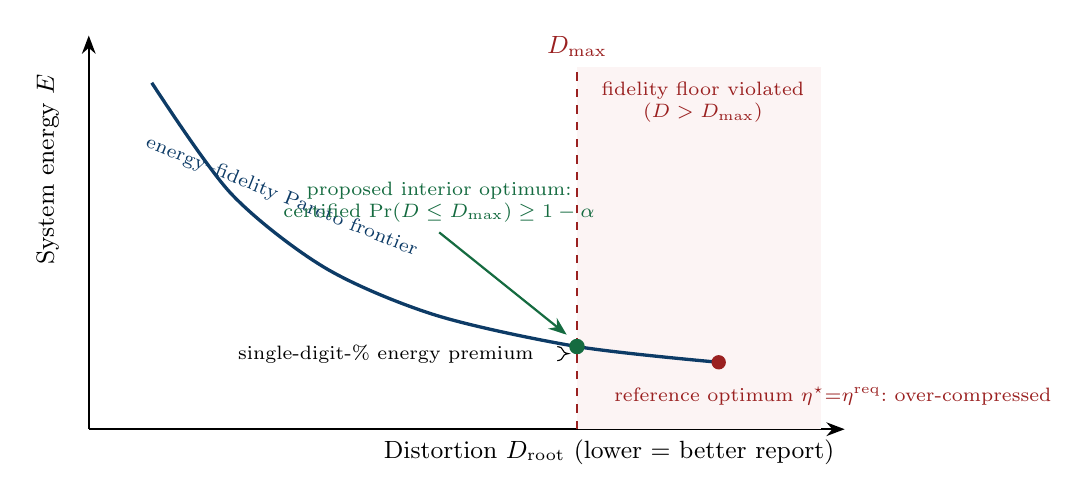
\begin{tikzpicture}[scale=1.0]
% axes
\draw[-{Stealth},thick] (0,0) -- (9.6,0) node[below left,font=\small]{Distortion $D_{\mathrm{root}}$ (lower = better report)};
\draw[-{Stealth},thick] (0,0) -- (0,5.0) node[rotate=90,anchor=south,font=\small,xshift=-1.7cm,yshift=0.25cm]{System energy $E$};
% infeasible region
\fill[palered] (6.2,0) rectangle (9.3,4.6);
\node[font=\scriptsize,text=brick,align=center] at (7.8,4.15) {fidelity floor violated\\($D>D_{\max}$)};
\draw[dashed,thick,brick] (6.2,0) -- (6.2,4.6) node[above,font=\small,text=brick]{$D_{\max}$};
% frontier
\draw[very thick,accent] plot[smooth] coordinates {(0.8,4.4) (1.8,3.0) (3.0,2.05) (4.4,1.45) (6.2,1.05) (8.0,0.85)};
\node[font=\scriptsize,text=accent,rotate=-22] at (2.45,2.95) {energy--fidelity Pareto frontier};
% reference point
\fill[brick] (8.0,0.85) circle (2.6pt);
\node[font=\scriptsize,text=brick,align=left,anchor=west] at (6.55,0.42) {reference optimum $\eta^{\star}{=}\eta^{\mathrm{req}}$:\ over-compressed};
% proposed point
\fill[okgreen] (6.2,1.05) circle (2.8pt);
\draw[-{Stealth},okgreen,thick] (4.45,2.5) node[above,font=\scriptsize,text=okgreen,align=center]{proposed interior optimum:\\ certified $\Pr(D\le D_{\max})\ge 1-\alpha$} -- (6.07,1.2);
% modest premium brace
\draw[decorate,decoration={brace,amplitude=4pt}] (5.95,1.05) -- (5.95,0.87) node[midway,left=5pt,font=\scriptsize]{single-digit-\% energy premium};
\end{tikzpicture}
\caption{Conceptual headline figure (F4) for \Dir{1}. Because the reference treats compression as free, its optimum slides past the fidelity floor; the proposed formulation operates \emph{at} $D_{\max}$, with the guarantee made distribution-free by conformal risk control \eqref{eq:crc}.}
\label{fig:pareto}
\end{figure}

\subsubsection{Tools, evaluation, contribution}
\textbf{Tools:} CVXPY (ECOS/SCS; MOSEK if licensed) extending the paper's BCD/SCA; OpenCOOD + one dataset; OpenCLIP/SigLIP; NumPy/SciPy. \textbf{Baselines:} the paper's own (No-Semantic, No-RAG, Max-Transmit-Power, Fixed-Speed, No-Motion). \textbf{Metrics:} the energy--fidelity Pareto frontier; certified coverage $\Pr(D\le D_{\max})$; mAP-anchored fidelity; energy saved by side-information-aware payloads versus the side-information-blind reference. \textbf{Contribution:} an information-theoretically grounded reformulation that overturns a published optimum, restores two classical theories (CEO, Wyner--Ziv) the model violates, derives $\eta^{\mathrm{req}}$ from first principles, and is the first in this line to carry a \emph{certified} fidelity guarantee and real-data calibration. Guaranteed floor: the reformulation alone is defensible even if every learned component slips.

% ----------------------------- D2 ---------------------------------
\subsection{Direction 2 (Rank 2) --- Learned, Decision-Focused Predictive Topology over a Provably Larger Action Space}
\label{sec:d2}

\begin{limitbox}{Targets: L9, L12, L19, L21, L22 (and the $\min(w_{ij},w_{ji})$ symmetrisation loss)}
The headline claim that the potential field ``overcomes short-sightedness'' rests on a single hand-tuned weight $\zeta$ whose mis-setting the paper's own Fig.~7 shows to be costly (L9); the field is evaluated post hoc at positions optimised without it (L19) around a centroid containing agents about to retire (L21); the matcher is exact but fed symmetrised weights; and the schedule is frozen to forced maximum parallelism in lockstep rounds (L12, L22). The per-round matcher (Edmonds' Blossom \cite{edmonds}) is \emph{already optimal} --- the suboptimality lives entirely in the \emph{edge weights and the action space}, which is exactly where learning and formulation repair belong.
\end{limitbox}

\begin{ideabox}{Key idea --- a four-stage algorithmic ladder, each stage a deliverable}
\textbf{Stage A ($\Phi$-in-the-loop; zero learning, repairs L19).} Move the lookahead \emph{inside} the inner problem: minimise $E^{\mathrm{total}}+\Phi_j$ in (P1). \textbf{Stage B (Lyapunov baseline; tuning-light).} Replace $\zeta$ by a drift-plus-penalty term from stochastic network optimisation \cite{neely}. \textbf{Stage C (learned cost-to-go).} Fitted value iteration for $\hat V_\theta$, optionally GNN-encoded, over directed weights. \textbf{Stage D (decision-focused fine-tuning).} Train \emph{through} the Blossom matcher so the loss is the realised multi-round energy, via blackbox differentiation of combinatorial solvers \cite{vlastelica,berthet}. All stages run over a \emph{flexible action space} that may idle pairs and vary depth (repairs L12/L22).
\end{ideabox}

\begin{remark}\label{rem:phiconvex}
Stage A is convexity-preserving: $\lVert\mathbf p-\mathbf c\rVert_2^{\delta}=(\lVert\mathbf p-\mathbf c\rVert_2^{2})^{\delta/2}$ is convex for $\delta\ge 2$ (convex increasing power of a convex non-negative function), and the data factor $L^{(k+1)}$ is constant within the motion block; the augmented inner problem therefore retains the paper's SCA/SOCP structure. Stage A is thus a one-week, zero-risk algorithm that fixes the paper's own internal inconsistency --- and gives the learned method a \emph{stronger} opponent to beat.
\end{remark}

\subsubsection{MDP formulation and learned weights}
Round evolution is a finite-horizon MDP: state $s^{(k)}=\{\mathbf p,\,L,\,\Omega,\,D\}$ of the active set; action $=$ a matching $\alpha^{(k)}\in\mathcal M(s^{(k)})$ \emph{including partial matchings} (idles allowed at any parity); stage cost $c(s,\alpha)=\sum_{(i,j)\in\alpha}E^{\mathrm{total}}_{(i,j)}\,(+\,\lambda\,\Delta D$ when composed with \Dir{1}). The augmented \emph{directed} edge weight is
\begin{equation}
w^{(k)}_{ij}=W^{(k)}_{ij}+\hat V_\theta\big(s^{(k+1)}\,\big|\,i\to j\big),
\label{eq:learnedw}
\end{equation}
solved each round by the same exact matcher; asymmetry is retained because L18 makes it principled. $\hat V_\theta$ is trained by fitted value iteration toward the Bellman target $\hat V_\theta(s)\approx\min_\alpha\{c(s,\alpha)+\hat V_{\bar\theta}(s')\}$ on simulator rollouts (stable, supervised; the deliberate choice is to learn a \emph{low-dimensional value}, not a combinatorial policy \cite{khalil,shen}), with an optional message-passing GNN encoder for size transfer (train at small $N$, deploy at $N{=}50$--$500$).

\begin{proposition}[Dominance of the flexible schedule]\label{prop:dominance}
Let $\mathcal A_{\mathrm{paper}}(s)$ be the matchings satisfying Eq.~(16b) (exactly $\lfloor N/2\rfloor$ pairs) and $\mathcal A_{\mathrm{flex}}(s)\supseteq\mathcal A_{\mathrm{paper}}(s)$ additionally allow idle agents at any parity and variable depth. For identical weights, the optimal cumulative cost over $\mathcal A_{\mathrm{flex}}$ is no greater than over $\mathcal A_{\mathrm{paper}}$; any strict improvement found by the learned policy is therefore a gain the published formulation cannot express. \emph{Proof:} minimisation over a superset. \hfill$\square$
\end{proposition}

\subsubsection{Decision-focused training (Stage D)}
Regressing $\hat V$ by mean-squared error optimises \emph{prediction} accuracy, but small errors near decision boundaries can flip the matching and incur large regret --- the canonical predict-then-optimize failure \cite{spo,mandi}. Stage D therefore fine-tunes $\theta$ on the \emph{decision loss}: the realised multi-round energy of the matched topology, with gradients passed through the Blossom solver by blackbox differentiation \cite{vlastelica} (informative linear-interpolation gradients for solvers of linear objectives --- matching qualifies) or perturbed optimisers \cite{berthet}. Stage C remains the stable fallback if Stage D underperforms within the schedule.

\begin{figure}[t]
\centering
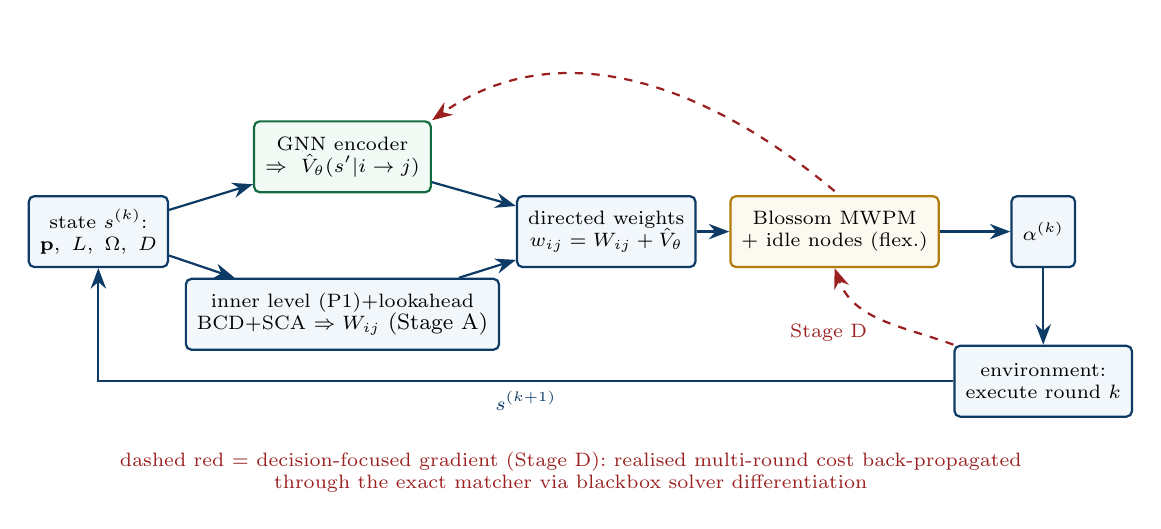
\begin{tikzpicture}[
  box/.style={draw=accent,fill=paleblue,thick,rounded corners=2pt,align=center,font=\scriptsize,inner sep=4pt,minimum height=9mm},
  gbox/.style={draw=okgreen,fill=palegreen,thick,rounded corners=2pt,align=center,font=\scriptsize,inner sep=4pt,minimum height=9mm},
  obox/.style={draw=gold,fill=palegold,thick,rounded corners=2pt,align=center,font=\scriptsize,inner sep=4pt,minimum height=9mm},
  arr/.style={-{Stealth[length=2.6mm]},thick,accent},
  garr/.style={-{Stealth[length=2.6mm]},thick,dashed,brick}]
\node[box] (state) at (0,0) {state $s^{(k)}$:\\ $\mathbf p,\ L,\ \Omega,\ D$};
\node[gbox] (gnn) at (3.1,0.95) {GNN encoder\\ $\Rightarrow\ \hat V_\theta(s'|i\to j)$};
\node[box] (inner) at (3.1,-1.05) {inner level (P1)+lookahead\\ BCD+SCA $\Rightarrow W_{ij}$ \footnotesize(Stage A)};
\node[box] (wts) at (6.45,0) {directed weights\\ $w_{ij}=W_{ij}+\hat V_\theta$};
\node[obox] (blossom) at (9.35,0) {Blossom MWPM\\ + idle nodes (flex.)};
\node[box] (act) at (12.0,0) {$\alpha^{(k)}$};
\node[box] (env) at (12.0,-1.9) {environment:\\ execute round $k$};
\draw[arr] (state) -- (gnn);
\draw[arr] (state) -- (inner);
\draw[arr] (gnn) -- (wts);
\draw[arr] (inner) -- (wts);
\draw[arr] (wts) -- (blossom);
\draw[arr] (blossom) -- (act);
\draw[arr] (act) -- (env);
\draw[arr] (env.west) -| node[pos=0.25,below,font=\scriptsize]{$s^{(k+1)}$} (state.south);
\draw[garr] (env.north west) to[out=160,in=-70] node[pos=0.55,below left=-1pt,font=\scriptsize,text=brick]{Stage D} (blossom.south);
\draw[garr] ($(blossom.north)+(0,0.05)$) to[out=140,in=35] (gnn.north east);
\node[font=\scriptsize,text=brick,align=center] at (6.0,-3.05) {dashed red $=$ decision-focused gradient (Stage D): realised multi-round cost back-propagated\\ through the exact matcher via blackbox solver differentiation};
\end{tikzpicture}
\caption{\Dir{2} pipeline. The exact matcher is retained; learning lives only in the edge weights. The dashed path is the Stage-D decision-focused gradient flowing through the solver back to the value network.}
\label{fig:pipeline}
\end{figure}

\subsubsection{Evaluation and contribution}
\textbf{Baselines:} tuned-$\zeta$ H--MAP, Stage-A $\Phi$-in-the-loop, Stage-B Lyapunov, Distance-Based, Pure-Greedy, Random, and a small-$N$ ($\le 8$) dynamic-programming \emph{optimality-gap oracle} the paper never reports. \textbf{Metrics:} cumulative energy; robustness with $\zeta$-tuning removed; generalisation across held-out geometries and sizes; wall-clock runtime to $N{=}500$ (first runtime-versus-$N$ curve for this framework, optionally accelerated by the amortised inner-solver surrogate of Sec.~\ref{sec:cross}). \textbf{Contribution:} dismantles the paper's named algorithmic novelty, repairs two of its internal inconsistencies for free (Stages A and the survivor centroid), and supplies a dominance guarantee plus the scalability the paper only claims --- the cleanest, most defensible ML narrative of the five.

% ----------------------------- D3 ---------------------------------
\subsection{Direction 3 (Rank 3) --- Trust-Aware, Byzantine-Resilient Semantic Aggregation}
\label{sec:d3}

\begin{limitbox}{Targets: L13 (with L8, L10, L17 touched)}
The tree has a structural single-path vulnerability: one hallucinating or adversarial leaf deterministically corrupts the global report, and $\Omega$ tracks provenance without integrity. Networked propagation of semantic corruption and Byzantine behaviour in LLM multi-agent systems are flagged as open problems in 2025--2026 \cite{securesemcom,sacbyz,decentllm,consensus}.
\end{limitbox}

\begin{ideabox}{Key idea --- overlap is redundancy, not just waste}
The paper uses spatial overlap $\rho$ only to \emph{discard} information (dedup). But agents whose patrol regions intersect can \emph{cross-validate} each other's claims on the shared region --- the same geometry that enables compression provides, for free, the redundancy needed for integrity verification.
\end{ideabox}

\textbf{Method.} Threat model: $f$ of $N$ agents inject corrupted/hallucinated payloads. Maintain a trust state $\tau_i\in[0,1]$ updated from \emph{consistency scores} $c_{ij}$ computed on region intersections (embedding agreement of the two agents' content restricted to $\mathcal R_i\cap\mathcal R_j$). Fusion becomes robust (reputation-weighted; geometric-median-style aggregation for numeric semantics, consistency-gated merging for symbolic content), and matching becomes trust-aware via $\tilde w_{ij}=w_{ij}+\mu(1-\tau_i)$ so suspicious sources are routed through verifying peers before reaching the root. Optionally add value-of-information weights $\nu_i$ and an AoI term \cite{aoi} (L8/L17). \textbf{Evaluation:} report-corruption rate versus $f$ versus energy overhead, against the trust-blind reference; resilience curves under dropout. \textbf{Contribution:} first integrity treatment for energy-optimised semantic aggregation trees; composes with \Dir{1} (corruption is adversarial distortion in the $\Theta$ state). Strong ``agentic-AI safety'' narrative; entirely simulation-feasible.

% ----------------------------- D4 ---------------------------------
\subsection{Direction 4 (Rank 4) --- Integrated Sensing and Communication (ISAC) Co-Design}
\begin{limitbox}{Targets: L1, L2}
A ``surveillance'' system whose mobility serves only the radio channel cannot reason about its mission: agents may drift toward the centroid (good communications) and away from their targets (poor sensing), and retired agents abandon their zones.
\end{limitbox}
\textbf{Method.} Add a position-dependent sensing-quality term --- a Cram\'er--Rao bound $\mathrm{CRB}_i(\mathbf p_i)\le\Gamma_i$ or detection-probability surrogate --- to the SCA motion planner, plus an idleness/coverage penalty $\Psi$ repairing L2, turning trajectories into an explicit three-way energy--channel--sensing compromise, in line with the 6G ISAC agenda for swarms \cite{isacswarm,admmisac}. \textbf{Evaluation:} sensing-versus-communication Pareto fronts; coverage quality over the horizon; demonstration that communication-only mobility measurably degrades sensing. Highest conceptual novelty for \emph{this} paper; demoted to rank 4 only because CRB-trajectory methodology is crowded, so the novelty is in the application.

% ----------------------------- D5 ---------------------------------
\subsection{Direction 5 (Rank 5) --- Robust Aggregation under Stochastic Channels}
\begin{limitbox}{Targets: L6}
The deterministic always-achievable Shannon rate is fragile for a contribution whose essence is ``move to improve the channel''; the authors concede the gap in their conclusion.
\end{limitbox}
\textbf{Method.} Rayleigh small-scale fading $h_{ij}=\beta_0\lVert\cdot\rVert^{-\delta}|g_{ij}|^2$, $g_{ij}\sim\mathcal{CN}(0,1)$; replace the deadline by the chance constraint $\Pr\{T^{\mathrm{mob}}+T^{\mathrm{comp}}+T^{\mathrm{comm}}\le T_{\max}\}\ge 1-\varepsilon$ via a safe Bernstein-type convex approximation that slots into the existing BCD/SCA machinery; model graceful degradation of semantic payloads versus the cliff effect. \textbf{Evaluation:} energy--reliability curves; deadline-violation rate of the paper's deterministic optimum under fading (expected to be material) versus the robust design meeting the target. Lowest risk of the five; the natural \emph{second} contribution stapled to \Dir{1}.

% ------------------------ wildcard + cross --------------------------
\subsection{Wildcard and Cross-Cutting Enhancements}
\label{sec:cross}
\textbf{Wildcard (rank 6) --- non-orthogonal / over-the-air semantic aggregation (L7, L10).} Replace orthogonal pairwise links with superposition-based fusion (AirComp / semantic feature multiple access), whose overhead is independent of the number of simultaneous senders. It is squarely in the reference paper's own lineage --- over-the-air feature fusion for integrated sensing and edge AI \cite{isea} and the April-2026 SFMA--ILAC thread that cites the reference and critiques purely orthogonal designs \cite{sfma} --- but it is a physical-layer redesign with synchronisation assumptions: too risky as the primary eight-week plan, ideal as scoped future work.

\textbf{Cross-cutting (bolt onto any direction).} (i) \emph{Modern ELM energy model} (L5, L15, L20): replace $\tau f^2 W$ by a prefill/decode-aware, memory-bandwidth-aware, mJ-per-token model \cite{edgellm,mei4llm} --- about one week, instantly defensible realism. (ii) \emph{Amortised inner solver} (L11): a permutation-equivariant GNN/MLP surrogate predicting $W_{ij}$ from pair features, labelled by the paper's own BCD/SCA, optionally physics-respecting via differentiable convex layers \cite{cvxpylayers}; this is the edge-weight engine that makes the $N{=}500$ runtime curve possible. (iii) \emph{Battery-aware objective} (L16): a min--max residual-energy variant reported alongside sum energy.

% =================== 5. COMPARATIVE ASSESSMENT ======================
\section{Comparative Assessment and Synergy}
\begin{table}[h]
\centering\footnotesize
\renewcommand{\arraystretch}{1.3}
\begin{tabular}{@{}c p{4.6cm} c c c c c@{}}
\toprule
\textbf{Rank} & \textbf{Core idea} & \textbf{Impact} & \textbf{Effort} & \textbf{ML depth} & \textbf{Eval.\ clarity} & \textbf{Risk} \\
\midrule
1 & Fidelity-aware CEO/WZ aggregation + conformal certification & High & Low--Med & Low--Med & Very high & Very low \\
2 & Learned decision-focused topology over flexible schedule & High & Medium & High & High & Low--Med \\
3 & Trust-aware Byzantine-resilient aggregation & High (freshest) & Medium & Medium & High & Medium \\
4 & ISAC sensing--communication co-design & Very high (concept) & Medium & Med (opt.) & High & Medium \\
5 & Chance-constrained robust channel & High (realism) & Low--Med & Med (opt.) & Very high & Very low \\
-- & Wildcard: AirComp/SFMA non-orthogonal fusion & Very high & High & Medium & Medium & High \\
\bottomrule
\end{tabular}
\caption{Comparative assessment. Ranks 1--2 are the recommended core; rank 3 is the freshest follow-up.}
\label{tab:compare}
\end{table}

\begin{infobox}{Why 1 + 2 compose into one coherent paper}
\Dir{1}'s Wyner--Ziv term makes pairwise costs asymmetric \emph{for a provable reason}; \Dir{2} retains directed weights to honour exactly that asymmetry; and the learned value $\hat V_\theta$ predicts remaining \emph{energy-plus-distortion}, so the topology becomes fidelity-aware end to end. Stage~A of \Dir{2} also repairs \Dir{1}'s solver environment (L19) before any learning is introduced. One narrative: \emph{fidelity-aware, learning-augmented progressive knowledge aggregation}.
\end{infobox}

% ====================== 6. EXECUTION PLAN ===========================
\section{Recommended Plan and Eight-Week Schedule}
\label{sec:plan}
\textbf{Primary line of work:} \Dir{1} as the non-negotiable foundation (guaranteed floor, theorem-overturning, certified) augmented by \Dir{2} as the algorithmic engine (dominance guarantee, ML narrative, scalability). For a maximum-freshness variant, swap Stage~D for a \Dir{3} prototype; for minimum risk, staple \Dir{5} to \Dir{1}.

\begin{table}[h]
\centering\footnotesize
\renewcommand{\arraystretch}{1.3}
\begin{tabular}{@{}c p{9.6cm} p{3.6cm}@{}}
\toprule
\textbf{Weeks} & \textbf{Milestones} & \textbf{Outputs} \\
\midrule
1--2 & Re-implement inner level (BCD+SCA, CVXPY) and outer level (Blossom, NetworkX); reproduce the paper's energy/scaling trends; set up OpenCOOD + dataset + VLM. & Faithful baseline; \textbf{F1} \\
3 & $\hat\rho$ pipeline; quantify geometric-vs-semantic mismatch; begin empirical rate--distortion curve. & \textbf{F2}; \textbf{F3} (start) \\
4 & Distortion state $\Theta$ (path-multiplicative), sub-additive fusion, Wyner--Ziv conditional payload; re-derive inner optimum ($\eta^{\star}$ interior); endogenous $\eta^{\mathrm{req}}$ lemma. & Theorem-overturning results; \textbf{F3} \\
5 & Constrained/scalarised solver; conformal calibration of the fidelity floor; sweep $D_{\max}/\lambda$ to trace the frontier. & \textbf{F4} (headline); \textbf{F8} \\
6 & Stage A $\Phi$-in-the-loop; Stage B Lyapunov baseline; flexible action space; MDP + fitted value iteration (optional GNN encoder). & Learned-topology module \\
7 & Full benchmarking (tuned-$\zeta$, Stage A/B, distance, greedy, random, small-$N$ DP oracle); $\zeta$-robustness; scaling and runtime to $N{=}500$; optional Stage-D decision-focused fine-tune. & \textbf{F5}, \textbf{F6} \\
8 & Ablations; polish figures; write report/manuscript. & \textbf{F7}; final report \\
\bottomrule
\end{tabular}
\caption{Eight-week execution plan (each phase concludes when its deliverable is achieved).}
\label{tab:weeks}
\end{table}

% ==================== 7. DELIVERABLES/TARGETS =======================
\section{Deliverables and Falsifiable Success Targets}
\label{sec:deliver}
\begin{table}[h]
\centering\footnotesize
\renewcommand{\arraystretch}{1.32}
\begin{tabular}{@{}p{4.4cm} p{10.6cm}@{}}
\toprule
\textbf{Deliverable} & \textbf{Concrete, falsifiable target} \\
\midrule
Reproduction baseline (repo) & Energy-vs-$N$ within a few percent of the paper's trend; same qualitative ordering of all benchmark schemes. \\
Fidelity-aware solver & Analytically and numerically: $\eta^{\star}<\eta^{\mathrm{req}}$ under a binding fidelity floor --- overturning the published trivial optimum. \\
Certified fidelity & Empirical coverage of $\Pr(D_{\mathrm{root}}\le D_{\max})\ge 1-\alpha$ on held-out runs via conformal risk control. \\
Side-information payload & Measurable energy reduction versus the side-information-blind reference at equal fidelity; report the saving as a function of overlap. \\
Proxy calibration ($\hat\rho$) & Correlation between geometric $\rho$ and measured $\hat\rho$, and \% of agent pairs whose redundancy ranking the geometric proxy inverts. \\
Energy--fidelity frontier & Reference optimum violates the floor by a measurable mAP/log-loss margin; proposed scheme meets it at a single-digit-\% energy premium. \\
Stage A ($\Phi$-in-the-loop) & Beats published H--MAP at equal tuning --- a repaired-inconsistency win requiring no learning. \\
Learned cost-to-go & Matches or beats the best hand-tuned $\zeta$ with \emph{zero} tuning on held-out geometries/sizes; never worse than forced parallelism (Prop.~\ref{prop:dominance}). \\
Optimality gap & First reported gap versus a small-$N$ ($\le 8$) dynamic-programming oracle. \\
Scalability (stretch) & End-to-end runs and runtime curve to $N\approx 100$--$500$; surrogate speed-up of order $100\times$ at a few-\% energy loss. \\
\bottomrule
\end{tabular}
\caption{Each headline claim is paired with the experiment and number that would confirm or refute it.}
\label{tab:targets}
\end{table}

\noindent\textbf{Deliverable figure list.} \textbf{F1} reproduction parity; \textbf{F2} geometric-vs-semantic mismatch scatter; \textbf{F3} empirical rate--distortion (mAP vs.\ $\eta$); \textbf{F4} energy--fidelity Pareto (headline, Fig.~\ref{fig:pareto}); \textbf{F5} cost-to-go vs.\ potential field across a $\zeta$ sweep (learned curve flat/lower); \textbf{F6} scalability: runtime and energy vs.\ $N$ to 500; \textbf{F7} ablations (geometry/semantics/hybrid $\hat\rho$; FVI vs.\ decision-focused; flexible vs.\ forced schedule); \textbf{F8} certified-coverage plot for \eqref{eq:crc}.

% ========================= 8. RISKS =================================
\section{Risk Management and Fallbacks}
\begin{itemize}
\item \textbf{Guaranteed floor (two independent wins requiring no learning):} \Dir{1}'s reformulation alone (interior optimum, sub-additive fusion, endogenous $\eta^{\mathrm{req}}$) and \Dir{2}'s Stage A ($\Phi$-in-the-loop). Either is a defensible project outcome by itself.
\item \textbf{If the Wyner--Ziv estimation is heavy:} fall back to the calibrated overlap-discount factor $\omega\hat\rho_{ij}$ in \eqref{eq:condpayload}; the conditional-rate floor remains as theory.
\item \textbf{If the learned value underperforms:} fitted value iteration before any GNN/RL; Stage B (Lyapunov) is already a deliverable, so the comparison story survives.
\item \textbf{If the VLM pipeline is heavy:} start $\hat\rho$ from shared-detection overlap before embeddings; the mismatch result (F2) still lands.
\item \textbf{Conformal layer:} statistically trivial to implement; near-zero risk, high defensibility.
\item \textbf{Spare near-certain win:} the chance-constrained fading channel (\Dir{5}), which the authors themselves flag, slots into the same BCD/SCA machinery.
\end{itemize}

% ====================== 9. PUBLICATION OUTLOOK ======================
\section{Publication Outlook}
The programme is framed honestly as an extension study; its novelty rests on checkable pieces benchmarked against the original. \Dir{1} --- a CEO/Wyner--Ziv-grounded reformulation that overturns a published optimum, restores side-information coding, and carries certified fidelity on real perception data --- targets \emph{IEEE Trans.\ Communications}, \emph{IEEE Trans.\ Cognitive Communications and Networking}, or \emph{IEEE IoT Journal}. \Dir{2} --- a decision-focused learned cost-to-go with a dominance guarantee, a repaired internal inconsistency, the first optimality-gap and runtime characterisations for this framework --- suits ICC/GLOBECOM or a wireless-ML workshop, and merges with \Dir{1} into one journal narrative. \Dir{3} is the natural follow-up paper riding the 2026 agentic-safety wave. The deliberate reuse of the paper's baselines, the small-$N$ exact oracle, and the conformal certificate are what make every headline number defensible under review.

% ========================== 10. CONCLUSION ==========================
\section{Conclusion}
The reference framework is a genuine contribution: it is the first to couple mobility, ELM-based semantic processing, and transmission for progressive knowledge aggregation in a single optimisable model. Precisely because it is clean, this audit could anchor twenty-three limitations --- five of them internal inconsistencies --- to specific equations, and convert them into five ranked, falsifiable research directions. The recommended core (fidelity-aware aggregation with certified guarantees, plus a learned, decision-focused topology over a provably larger schedule space) overturns a published optimum, repairs two inconsistencies at zero risk, restores two classical information-theoretic principles the model violates, and supplies the scalability and optimality-gap evidence the paper only claims --- a programme with a guaranteed floor, a high ceiling, and a clear path to publication.

% ========================== REFERENCES ==============================
\begin{thebibliography}{99}\footnotesize
\bibitem{refpaper} Z.~Zhao, J.~Wang, Z.~Yang, K.~Yang, Z.~Zhang, M.~Chen, K.~Huang, ``Agentic AI--empowered wireless agent networks with semantic-aware collaboration via ILAC,'' arXiv:2604.02381, 2026.
\bibitem{ceo} T.~Berger, Z.~Zhang, H.~Viswanathan, ``The CEO problem,'' \emph{IEEE Trans.\ Inf.\ Theory}, 42(3), 1996.
\bibitem{courtade} T.~A.~Courtade, T.~Weissman, ``Multiterminal source coding under logarithmic loss,'' \emph{IEEE Trans.\ Inf.\ Theory}, 60(1), 2014.
\bibitem{wynerziv} A.~Wyner, J.~Ziv, ``The rate-distortion function for source coding with side information at the decoder,'' \emph{IEEE Trans.\ Inf.\ Theory}, 22(1), 1976.
\bibitem{blau} Y.~Blau, T.~Michaeli, ``Rethinking lossy compression: the rate--distortion--perception tradeoff,'' \emph{ICML}, 2019.
\bibitem{stavrou} P.~A.~Stavrou, M.~Kountouris, ``The role of fidelity in goal-oriented semantic communication: a rate--distortion approach,'' \emph{IEEE Trans.\ Commun.}, 71(7), 2023.
\bibitem{rdpsem} X.~Niu \emph{et al.}, ``Rate--distortion--perception theory for semantic communication,'' arXiv:2312.05437, 2023.
\bibitem{semantic_ic} ``SemantIC: semantic interference cancellation towards 6G,'' arXiv:2310.12768 (\emph{IEEE Commun.\ Lett.}), 2024.
\bibitem{wzcodebook} ``A Wyner--Ziv coding-based semantic communication approach with a shared semantic codebook,'' \emph{IEEE} (Xplore 10464918), 2024.
\bibitem{rdo} ``Rate--distortion optimized communication for collaborative perception,'' arXiv:2509.21994, 2025.
\bibitem{where2comm} Y.~Hu \emph{et al.}, ``Where2comm: communication-efficient collaborative perception via spatial confidence maps,'' \emph{NeurIPS}, 2022.
\bibitem{cods} ``CoDS: collaborative perception via digital semantic communication,'' arXiv:2512.22513, 2025.
\bibitem{scomcp} ``SComCP: task-oriented semantic communication for collaborative perception,'' arXiv:2507.00895, 2025.
\bibitem{opv2v} R.~Xu \emph{et al.}, ``OPV2V: an open benchmark and fusion pipeline for V2V perception,'' \emph{ICRA}, 2022.
\bibitem{v2xsim} Y.~Li \emph{et al.}, ``V2X-Sim,'' \emph{IEEE Robot.\ Autom.\ Lett.}, 2022.
\bibitem{zecchin} M.~Zecchin, O.~Simeone, ``Online conformal compression for zero-delay communication with distortion guarantees,'' arXiv:2503.08340, 2025.
\bibitem{ppc} ``Prediction-powered communication with distortion guarantees,'' arXiv:2509.24373, 2025.
\bibitem{confsensor} M.~Zhu \emph{et al.}, ``Conformal distributed remote inference in sensor networks under reliability and communication constraints,'' \emph{IEEE Trans.\ Signal Process.}, 73, 2025.
\bibitem{cohen} K.~M.~Cohen, S.~Park, O.~Simeone, S.~Shamai, ``Calibrating AI models for wireless communications via conformal prediction,'' \emph{IEEE TMLCN}, 1, 2023.
\bibitem{ltt} A.~N.~Angelopoulos \emph{et al.}, ``Learn then test: calibrating predictive algorithms to achieve risk control,'' \emph{Ann.\ Appl.\ Stat.}, 19(2), 2025.
\bibitem{spo} A.~N.~Elmachtoub, P.~Grigas, ``Smart `predict, then optimize','' \emph{Management Science}, 68(1), 2022.
\bibitem{mandi} J.~Mandi \emph{et al.}, ``Decision-focused learning: foundations, state of the art, benchmark and future opportunities,'' \emph{JAIR}, 2024.
\bibitem{vlastelica} M.~Vlastelica, A.~Paulus, V.~Musil, G.~Martius, M.~Rol\'inek, ``Differentiation of blackbox combinatorial solvers,'' \emph{ICLR}, 2020.
\bibitem{berthet} Q.~Berthet \emph{et al.}, ``Learning with differentiable perturbed optimizers,'' \emph{NeurIPS}, 2020.
\bibitem{cvxpylayers} A.~Agrawal \emph{et al.}, ``Differentiable convex optimization layers,'' \emph{NeurIPS}, 2019.
\bibitem{khalil} E.~Khalil \emph{et al.}, ``Learning combinatorial optimization algorithms over graphs,'' \emph{NeurIPS}, 2017.
\bibitem{shen} Y.~Shen, Y.~Shi, J.~Zhang, K.~B.~Letaief, ``Graph neural networks for scalable radio resource management,'' \emph{IEEE JSAC}, 39(1), 2021.
\bibitem{neely} M.~J.~Neely, \emph{Stochastic Network Optimization with Application to Communication and Queueing Systems}, Morgan \& Claypool, 2010.
\bibitem{edmonds} J.~Edmonds, ``Paths, trees, and flowers,'' \emph{Canad.\ J.\ Math.}, 17, 1965.
\bibitem{tokcom} L.~Qiao \emph{et al.}, ``Token communications: a unified framework for cross-modal context-aware semantic communications,'' arXiv:2502.12096, 2025.
\bibitem{mltok} ``Machine-language tokens for task-oriented agent communication,'' arXiv:2507.21454, 2025.
\bibitem{c2c} ``Cache-to-Cache: direct semantic communication between large language models,'' arXiv:2510.03215, 2025.
\bibitem{latentsurvey} ``Beyond tokens: latent-space communication among AI agents,'' arXiv:2606.05711, 2026.
\bibitem{securesemcom} ``Secure semantic communications: threats, countermeasures, and open challenges,'' arXiv:2602.22134, 2026.
\bibitem{sacbyz} ``Byzantine-robust multi-agent LLM systems via semantic anomaly checking,'' arXiv:2605.09076, 2026.
\bibitem{decentllm} ``DecentLLMs: decentralized Byzantine-tolerant coordination of LLM agents,'' arXiv:2507.14928, 2025.
\bibitem{consensus} ``ConSensus: hybrid semantic--statistical consensus for unreliable multi-agent fusion,'' arXiv:2601.06453, 2026.
\bibitem{isea} Z.~Liu, Q.~Lan, K.~Huang \emph{et al.}, ``Over-the-air fusion of sparse spatial features for integrated sensing and edge AI,'' arXiv:2404.17973, 2024.
\bibitem{sfma} J.~Wang \emph{et al.}, ``Semantic feature multiple access empowered integrated learning and communication networks,'' arXiv:2604.09255, 2026.
\bibitem{edgellm} ``Edge inference for large language models: measurements, energy models, and optimization,'' arXiv:2604.22906, 2026.
\bibitem{mei4llm} Z.~Lin \emph{et al.}, ``Pushing large language models to the 6G edge: vision, challenges, and opportunities,'' arXiv:2407.18921, 2024.
\bibitem{aoi} R.~D.~Yates \emph{et al.}, ``Age of information: an introduction and survey,'' \emph{IEEE JSAC}, 39(5), 2021.
\bibitem{isacswarm} Y.~Ma \emph{et al.}, ``Integrated sensing, communication, computing, and control meets UAV swarms in 6G,'' arXiv:2512.07054, 2025.
\bibitem{admmisac} Z.~Zhai \emph{et al.}, ``Integrated sensing and communication with UAV swarms via decentralized consensus ADMM,'' arXiv:2511.03283, 2025.
\end{thebibliography}

\vspace{0.6em}
\begin{center}\footnotesize\itshape
This document is a critical review and research proposal prepared for academic discussion.\\ All external claims are attributed to the cited literature; all equation anchors refer to the reference paper \cite{refpaper}.
\end{center}

\end{document}
